\documentclass{article}

\usepackage[margin=1.5in]{geometry}
\usepackage{amsmath}
\usepackage{listings}
\usepackage{color}
\usepackage{placeins}
\usepackage{graphicx}
\graphicspath{ {/home/sajid/Desktop/Computational-Economics/Problem Set 1} }

\title{Computational Economics: Problem Set 1}
\author{S M Sajid Al Sanai}
\date{May 1, 2019}

\begin{document}

\maketitle
\pagenumbering{arabic}
\tableofcontents

\lstset{
	frame=lines,
	basicstyle=\small\sffamily,
	tabsize=4,
	columns=fixed,
	showstringspaces=false,
	showtabs=false,
	keepspaces,
	commentstyle=\color{red},
	keywordstyle=\color{blue}
}

\newpage

\section{Infinite Horizon Ramsey Model}

\subsection{Value Function Approximation}

\subsubsection{Bellman Equation}

\noindent Given our Maximisation Problem,

\begin{equation}
max_{\{ K_t \}_{t=1} ^{\infty} } \sum_{t=0} ^{\infty} \beta^t u(C_t)
\end{equation}

\noindent Where our Utility Function is specified,

\begin{equation}
u(C_t) = \ln(C_t)
\end{equation}

\noindent Where our Production Function is specified,

\begin{equation}
F(K_t) = AK^{\alpha} _t
\end{equation}

\noindent Given $K_0$ and Non-Negativity Constraints,

\begin{equation}
C_t,K_{t+1}\geq 0
\end{equation}

\noindent Given Law of Motion of Capital,

\begin{equation}
I_t=K_{t+1}-(1-\delta)K_t
\end{equation}

\noindent Given Budget Constraint limited by the Production Function,

\begin{equation}
F(K_t)\geq C_t + I_t
\end{equation}

\noindent Derive our Consumption and summarise our Production,

\begin{equation}
C_t = F(K_t)-K_{t+1}+(1-\delta)K_t
\end{equation}

\begin{equation}
f(K_t) = F(K_t)+(1-\delta)K_t
\end{equation}

\begin{equation}
\implies C_t=f(K_t)-K_{t+1}
\end{equation}

\noindent Substituting Consumption into our Maximisation Problem allows us to derive our Bellman Equation,

\begin{equation}
V( K_t ) = max_{ \{ K_{t+1} \} } u( f(K_t) - K_{t+1} ) + \beta V(K_{t+1})
\end{equation}

\begin{equation}
V( K_t ) = max_{ \{ K_{t+1} \} } \ln( AK^{\alpha} _t - (1-\delta)K_t - K_{t+1} ) + \beta V(K_{t+1})
\end{equation}

\newpage

\subsubsection{Value Function Iteration}

Value Function Iteration conducted over the discretised space for Capital assuming $\beta=0.6, \ A=20, \ \alpha=0.3,$ and $\delta=0.5$ yields the following graph visualising output,

\begin{figure}[h]
\begin{center}
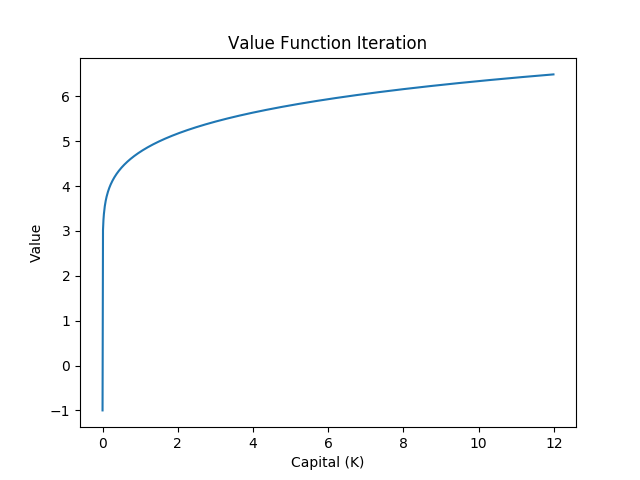
\includegraphics[width=\textwidth]{Figure1.png}
\caption{Value Function Iteration over Discretised Capital}
\end{center}
\end{figure}
\FloatBarrier

\newpage

\subsection{Customised Value Function Approximation}

\subsubsection{Using Iteration}

Value Function Iteration conducted over the discretised space for Capital assuming $\beta=0.6, \ A=1, \ \alpha=0.3,$ and $\delta=1$ yields the following graph visualising output,

\begin{figure}[h]
\begin{center}
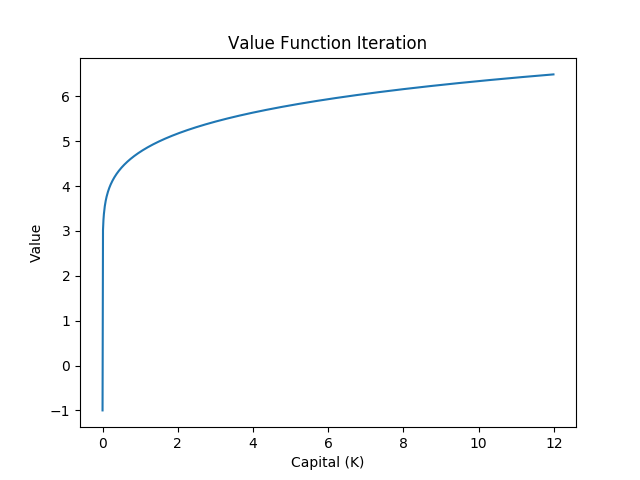
\includegraphics[width=\textwidth]{Figure1.png}
\caption{Value Function Iteration over Discretised Capital}
\end{center}
\end{figure}
\FloatBarrier

\newpage

\subsubsection{Using Analytical Form}

Value Function Iteration conducted over the discretised space for Capital assuming $\beta=0.6, \ A=1, \ \alpha=0.3,$ and $\delta=1$ is superimposed with the Analytical Form for comparison of output,

\begin{figure}[h]
\begin{center}
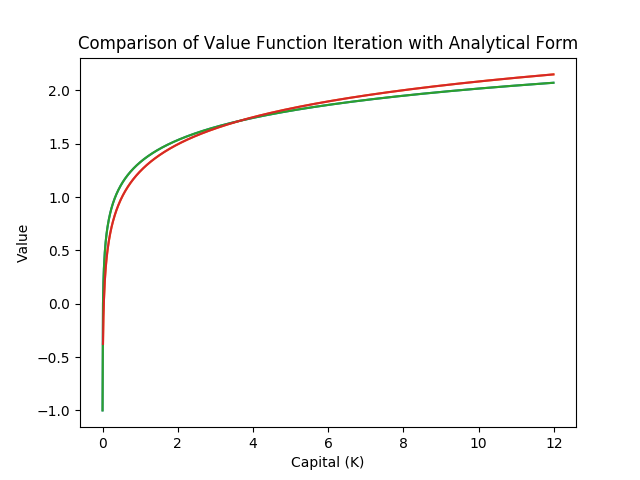
\includegraphics[width=\textwidth]{Figure3.png}
\caption{Comparison of Value Function Iteration with Analytical Form}
\end{center}
\end{figure}
\FloatBarrier

With our initial guess of the functional form of the analytical form being,

\begin{equation}
V(K_t) = A + B \ln K_t
\end{equation}

\begin{equation}
\implies A = \frac{\alpha \beta}{1- \alpha \beta} \ln \alpha \beta
\end{equation}

\begin{equation}
\implies B=\frac{\alpha}{1-\alpha\beta}
\end{equation}

\newpage

\section{Rust Model}

% Code Snippet
\begin{lstlisting}
Estimation of Parameters and respective Standard Errors:
Beta[0]:     [25.36425337]; (0.11561192456479381) 0.013366117101575576
Beta[1]:     [-1.48315299]; (3.004018606720816) 9.024127789524872
Beta[2]:     [0.18493143]; (0.04011846630681128) 0.001609491338810752
Alpha:       [-8.37344604]; (0.003586413934865264) 1.2862364912195745e-05
Sigma Alpha: [1.075]; (1.265210529517815) 1.6007576840027502
\end{lstlisting}

\newpage

\section{Appendix}

\subsection{Source}

\subsubsection{Source: Question 1}

\lstinputlisting[language=Python]{pset1_1_source.py}

\newpage

\subsubsection{Source: Question 2}

\lstinputlisting[language=Python]{pset1_2_source.py}

\newpage

\subsection{Output}

\lstinputlisting{pset1_output.txt}

\end{document}